\documentclass[a4paper,12pt]{article}
\usepackage[a4paper,top=1.3cm,bottom=2cm,left=1.5cm,right=1.5cm,marginparwidth=0.75cm]{geometry}
\usepackage{cmap}
\usepackage{mathtext}
\usepackage[T2A]{fontenc}
\usepackage[utf8]{inputenc}
\usepackage[english,russian]{babel}
\usepackage{siunitx}
\usepackage{enumitem}
\usepackage{placeins}

\usepackage{graphicx}
\usepackage{amsmath}

\usepackage{wrapfig}
\usepackage{tabularx}
\usepackage{multirow}

\usepackage{hyperref}
\usepackage[rgb]{xcolor}
\hypersetup{colorlinks=true,urlcolor=blue}
\usepackage{siunitx}
\usepackage{amsmath,amsfonts,amssymb,amsthm,mathtools}
\usepackage{mathtools}
\usepackage{icomma}
\mathtoolsset{showonlyrefs=false}
\usepackage{euscript}
\usepackage{mathrsfs}
\DeclareMathOperator{\sgn}{\mathop{sgn}}
\newcommand*{\hm}[1]{#1\nobreak\discretionary{}
{\hbox{$\mathsurround=0pt #1$}}{}}

%%% Заголовок
\newcommand\labname{Исследование энергетического спектра $\beta$-частиц и определение их максимальной энергии при помощи магнитного спектрометра}
\newcommand\labnumber{4.2}


\author{Макаров Лев Евгеньевич}
\title{Лабораторная работа №\labnumber

\labname
}

\date{\today}

\begin{document}

\begin{titlepage}
	\begin{center}
		{\large МОСКОВСКИЙ ФИЗИКО-ТЕХНИЧЕСКИЙ ИНСТИТУТ (НАЦИОНАЛЬНЫЙ ИССЛЕДОВАТЕЛЬСКИЙ УНИВЕРСИТЕТ)}
	\end{center}
	\begin{center}
		{\large Физтех-школа фотоники, электроники и молекулярной физики}
	\end{center}
	
	
	\vspace{4.5cm}
	{\huge
		\begin{center}
			{\bf Отчёт о выполнении лабораторной работы \labnumber}\\
			\labname
		\end{center}
	}
	\vspace{2cm}
	\begin{flushright}
		{\LARGE Автор:\\ Макаров Лев Евгеньевич \\
			\vspace{0.2cm}
			Б04-306}
	\end{flushright}
	\vspace{8cm}
	\begin{center}
		Долгопрудный 2025
	\end{center}
\end{titlepage}

\section{Введение}

\textbf{Цель работы:} 
\begin{enumerate}
	\item С помощью магнитного спектрометра исследовать энергетический спектр $\beta$-частиц при распаде ядер $\prescript{137}{}{\text{Cs}}$
    \item Определить их максимальную энергию
\end{enumerate}

\section{Теоретические сведения}

Бета-распад - самопроизвольное превращение ядер, при котором их массовое число не изменяется, а заряд увеличивается или уменьшается на единицу. Бета-активные ядра встречаются во всей области значений массового числа $A$, начиная от единицы (свободный нейтрон) и кончая самыми тяжелыми ядрами. Выделяющаяся при единичном акте $\beta$-распада энергия варьируется от 18 кэВ (для распада трития $\prescript{3}{1}{\text{H}}$) до 13,4 МэВ (для распада изотопа бора $\prescript{12}{5}{\text{B}}$).

В данной работе мы будем иметь дело с электронным распадом

\begin{equation*}
    \prescript{A}{Z}{X} \to \prescript{A}{Z+1}{X} + e^{-} + \tilde{\nu}
\end{equation*}

при котором кроме электрона испускается антинейтрино. Освобождающаяся при $\beta$-распаде энергия делится между электроном, антинейтрино и дочерним ядром, однако доля энергии, передаваемой ядру, исчезающе мала по сравнению с энергией, уносимой электроном и антинейтрино. Практически можно считать, что эти две частицы делят между собой всю освобождающуюся энергию. Поэтому электроны могут иметь любое значение энергии — от нулевой до некоторой максимальной, которая равна энергии, освобождающейся при $\beta$-распаде, являющейся важной физической величиной.

Вероятность $d w$ того, что при распаде электрон вылетит с импульсом $d^3 \mathbf{p}$, а антинейтрино с импульсом в интервале $d^3 \mathbf{k}$, очевидно, пропорциональна произведению этих дифференциалов. Но мы должны еще учесть закон сохранения энергии, согласно которому импульсы $\mathbf{p}$ и $\mathbf{k}$ электрона и антинейтрино связаны соотношением

\begin{equation}\label{eq:1}
    E_e - E - ck = 0
\end{equation}


где $E_e$ — максимальная энергия электрона, кинетическая энергия электрона $E$ связана с его импульсом обычным релятивистским соотношением

\begin{equation}\label{eq:2}
    E = c \sqrt{p^2 + m^2 c^2} - mc^2
\end{equation}


а через $ck$ обозначена энергия антинейтрино с импульсом $k$. Условие \eqref{eq:1} можно учесть введением в выражение для $dw$ $\delta$-функции

\begin{equation}\label{eq:3}
    \delta \left( E_e - E - ck \right)
\end{equation}

по определению не равной нулю только при соблюдении условия \eqref{eq:1}.

Таким образом, вероятность $dw$ может быть записана в виде

\begin{equation}\label{eq:4}
    dw = D \delta \left( E_e - E - ck \right) d^3 \mathbf{p} d^3 \mathbf{k} = D \delta \left( E_e - E - ck \right) p^2 dp k^2 dk \ d\Omega_e d \Omega_{\tilde{\nu}}
\end{equation}

где $D$ — некоторый коэффициент пропорциональности, $d \Omega_e$, $d \Omega_{\tilde{\nu}}$ — элементы телесных углов направлений вылета электрона и нейтрино. Вероятность $dw$ непосредственно связана с $\beta$-спектром, поскольку для очень большого числа $N_0$ распадов число $dN$ распадов с вылетом электрона и антинейтрино с импульсом соответственно от $\mathbf{p}$ до $\mathbf{p} + d\mathbf{p}$ и от $\mathbf{k}$ до $\mathbf{k} + d\mathbf{k}$ определяется соотношением


\begin{equation}\label{eq:5}
    dN = N_0 dw
\end{equation}


Коэффициент $D$ в формуле \eqref{eq:4} можно считать для рассматриваемых нами так называемых разрешенных фермиевских типов распадов с хорошей точностью константой (разрешенными называются такие переходы, при которых не изменяются ни момент, ни четность состояния ядра). В этом случае величину $dw$ из \eqref{eq:5} можно проинтегрировать по всем углам и по абсолютному значению импульса нейтрино. Интегрирование по каждому телесному углу дает множитель $4 \pi$, а интегрирование по $dk$ проводится с использованием основного свойства $\delta$-функции


\begin{equation}\label{eq:6}
    \int\limits_{-\infty}^{+\infty} f(x) \delta(x) dx = f(0)
\end{equation}

Поэтому при интегрировании по $k$ $\delta$-функция исчезнет, а $ck$ всюду заменится на $(E_e - E)$. После умножения на полное число распадов $N_0$ проинтегрированное выражение приобретает смысл числа электронов $dN$, вылетающих из ядра с импульсом, абсолютная величина которого лежит между $p$ и $p + dp$:

\begin{equation}\label{eq:7}
    dN = \frac{16 \pi^2 N_0 }{c^2} D p^2 \left( E_e - E \right)^2 dp
\end{equation}

Чтобы получить распределение электронов не по импульсам, а по энергиям, надо в \eqref{eq:7} перейти от $dp$ к $dE$:

\begin{equation}\label{eq:8}
    dE = \frac{c^2 p}{E + mc^2}dp
\end{equation}


после чего выражающая форму $\beta$-спектра величина $N (E) = dN/dE$ приобретает вид

\begin{equation}\label{eq:9}
    \frac{dN}{dE} = N_0 B cp \left( E + mc^2 \right) \left( E_e - E \right)^2 = N_0 B \sqrt{E \left( E + 2mc^2 \right)} \left( E_e - E \right)^2 \left( E + mc^2 \right)
\end{equation}

где $B = (16 \pi^2/c^4)D$. В нерелятивистском приближении, которое и имеет место с нашем случае, выражение \eqref{eq:9} упрощается, и мы имеем

\begin{equation} \label{eq:10}
    \frac{dN}{dE} \approx \sqrt{E} \left( E_e - E \right)^2
\end{equation}

\FloatBarrier
\begin{figure}[h]
    \begin{center}
        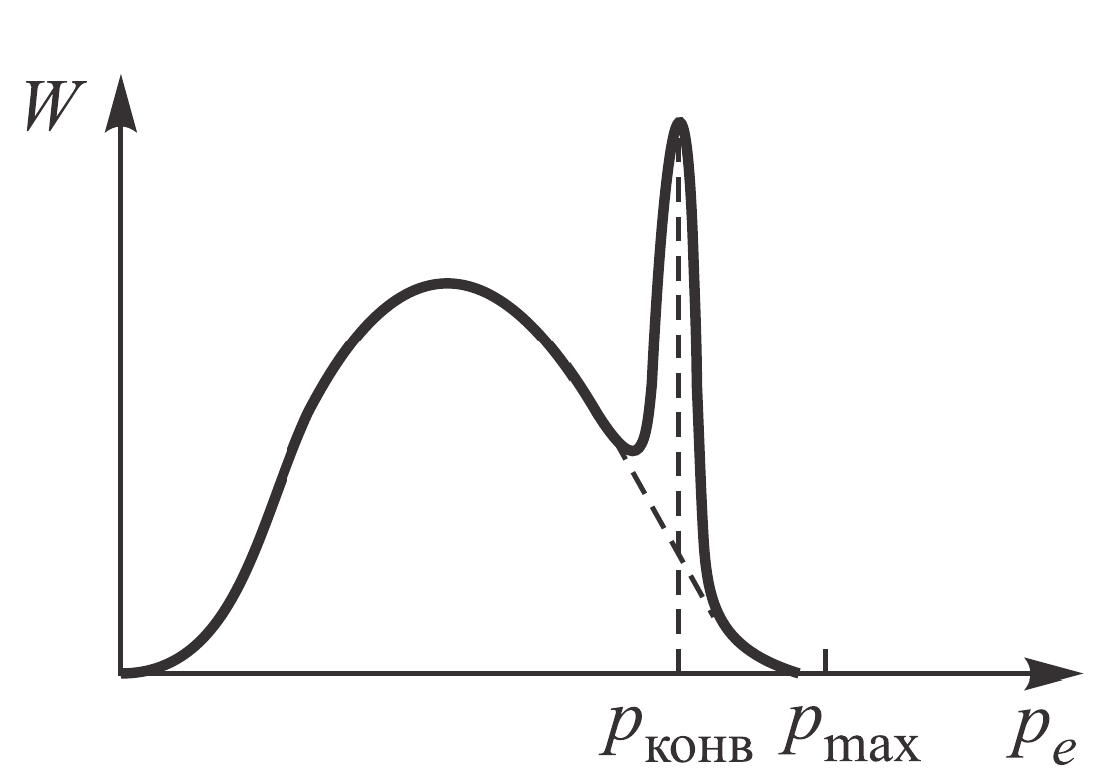
\includegraphics[width = 0.45\textwidth]{pics/beta_specter.png}
        \caption{Форма спектра $\beta$-частиц при разрешенных переходах}
    \label{pic:beta_specter}
    \end{center}
\end{figure}
\FloatBarrier

Выражение \eqref{eq:10} приводит к спектру, имеющему вид широкого колокола (см. рис. \ref{pic:beta_specter}). Кривая плавно отходит от нуля и столь же плавно, по параболе, касается оси абсцисс в области максимальной энергии электронов $E_e$.

Дочерние ядра, возникающие в результате $\beta$-распада, нередко оказываются возбужденными. Возбужденные ядра отдают свою энергию либо излучая $\gamma$-квант (энергия которого равна разности энергий начального и конечного уровней), либо передавая избыток энергии одному из электронов с внутренних оболочек атома. Излучаемые в таком процессе электроны имеют строго определенную энергию и называются конверсионными.

Конверсия чаще всего происходит на оболочках $K$ или $L$. На спектре, представленном на рис. \ref{pic:beta_specter}, видна монохроматическая линия, вызванная электронами конверсии. Ширина этой линии в нашем случае является чисто аппаратурной — по ней можно оценить разрешающую силу спектрометра.

\section{Экспериментальная установка}

\FloatBarrier
\begin{figure}[h]
    \begin{center}
        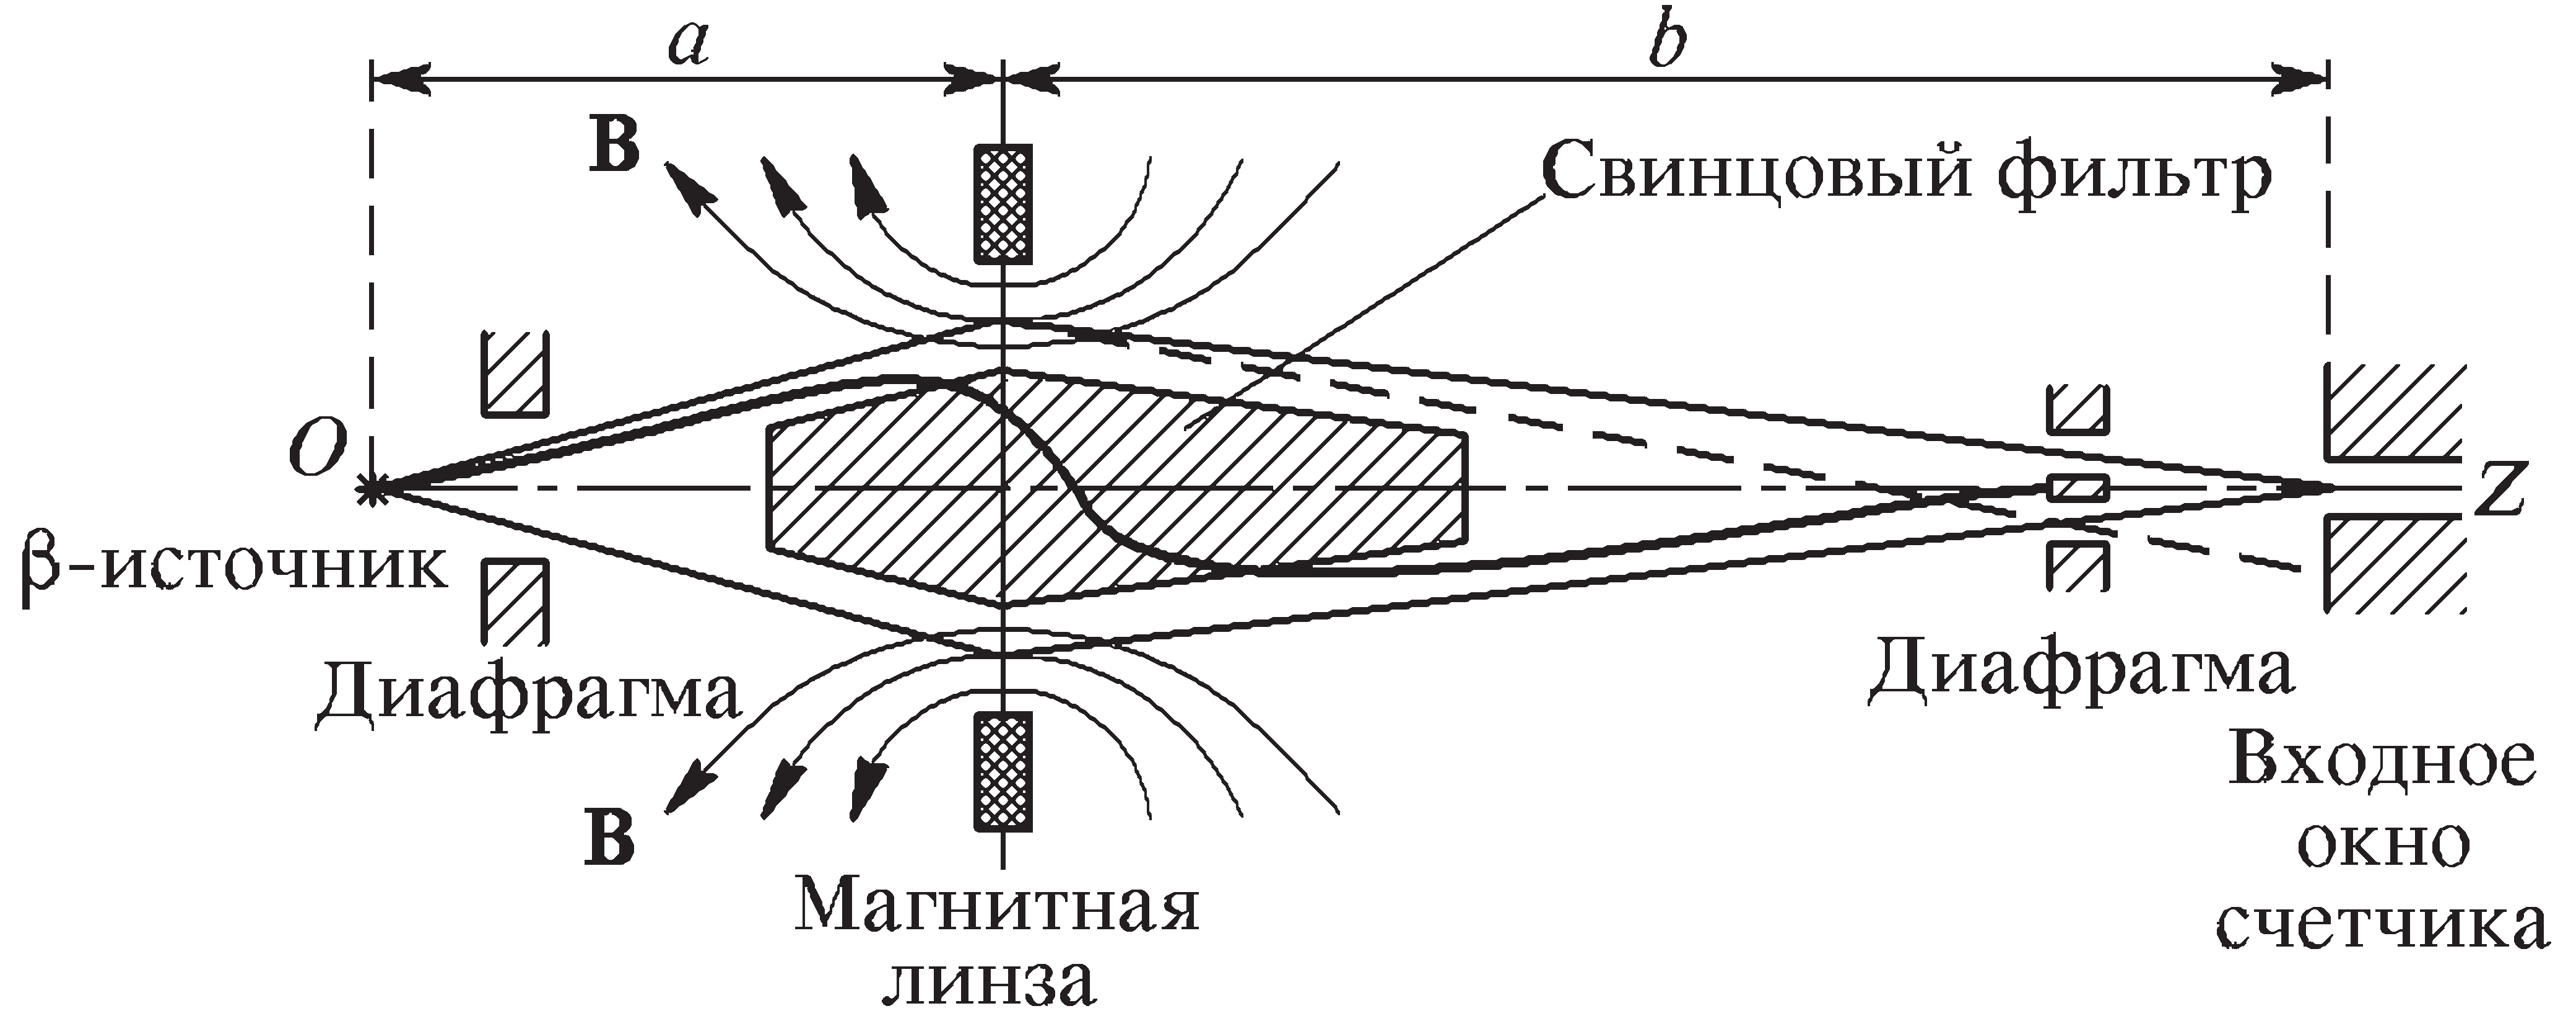
\includegraphics[width = 1\textwidth]{pics/ustan_1.png}
        \caption{Схема $\beta$-спектрометра с короткой магнитной линзой}
    \label{pic:ustan-1}
    \end{center}
\end{figure}
\FloatBarrier

Энергию $\beta$-частиц определяют с помощью $\beta$-спектрометров. В работе используется магнитный спектрометр с «короткой линзой». Электроны, испускаемые радиоактивным источником (рис. \ref{pic:ustan-1}), попадают в магнитное поле катушки, ось которой параллельна оси $OZ$ (оси симметрии прибора). Траектории электронов в магнитном поле представляют собой схематически показанные на рисунке сложные спирали, сходящиеся за катушкой в фокусе, расположенном на оси $OZ$. Силовые линии магнитного поля изображены на рис. \ref{pic:ustan-1} тонкими линиями. В фокусе установлен детектор электронов — газоразрядный торцевой счетчик с тонким входным окном, прозрачным для электронов с энергией больше 40 кэВ, либо сцинтилляционный счетчик. Чувствительным элементом сцинтилляционного счетчика является тонкий кристалл полистирола. При попадании электрона в кристалле возникает световая вспышка — сцинтилляция, регистрируемая фотоумножителем. Принципы работы сцинтиллятора и фотоумножителя описаны в Приложениях II и III.

Как показывает расчет, для заряженных частиц тонкая катушка эквивалентна линзе. Ее фокусное расстояние $f$ зависит от импульса электронов $p_e$ и от индукции магнитного поля линзы (т. е. от силы тока $I$, протекающего через катушку) следующим образом:

\begin{equation}\label{eq:11}
    \frac{1}{f} \propto \frac{I^2}{p_e^2}
\end{equation}


При заданной силе тока на входное окно счетчика фокусируются электроны с определенным импульсом. Электроны, обладающие другими значениями импульса, при этом не сфокусированы и в основном проходят мимо окна (штриховой луч). При изменении тока в катушке на счетчик последовательно фокусируются электроны с разными импульсами. Так как геометрия прибора в течение всего опыта остается неизменной, импульс сфокусированных электронов пропорционален величине тока $I$:


\begin{equation}\label{eq:12}
    p_e = kI
\end{equation}

Константа прибора $k$ обычно определяется не из расчета, а из опыта (по какой-нибудь известной конверсионной линии).


Короткая магнитная линза обладает заметной сферической аберрацией, т. е. имеет разные фокусные расстояния для частиц, вылетающих из источника под различными углами. Поэтому приходится устанавливать кольцевые диафрагмы, ограничивающие углы вылета электронов, как это изображено на рис. \ref{pic:ustan-1}. Свинцовый фильтр предохраняет счетчик от прямого попадания $\gamma$-лучей, почти всегда сопровождающих $\beta$-распад. Из-за конечных размеров источника, диафрагм и окна счетчика, а также вследствие аберраций при заданной величине фокусного расстояния на счетчик попадают электроны с импульсами, лежащими внутри некоторого интервала от $p_e - \Delta p_e/2$ до $p_e + \Delta p_e/2$. Величина $\Delta p_e$ — ширина интервала импульсов, регистрируемых при заданном значении тока, — называется разрешающей способностью $\beta$-спектрометра. Из рис. \ref{pic:ustan-1} ясно, что разрешающая способность спектрометра зависит от того, какой угол с осью $OZ$ составляют регистрируемые электроны. Электроны, летящие под небольшим углом к оси спектрометра, практически не отклоняются магнитным полем и попадали бы в окно $\beta$-счетчика при любом токе в линзе, если бы на их пути не было свинцового фильтра. Поэтому разрешение спектрометра зависит не только от размеров кольцевых диафрагм, но и от диаметра свинцового фильтра.

Рассмотрим теперь связь между числом частиц, регистрируемых установкой, и функцией $W (p_e) = dW/dp_e$, определяемой формулой \eqref{eq:10}. Как легко понять,

\begin{equation}\label{eq:13}
    N (p_e) \simeq W(p_e) \Delta p_e
\end{equation}

где $\Delta p_e$ — разрешающая способность спектрометра. Формула \eqref{eq:11} показывает, что при заданном токе фокусное расстояние магнитной линзы зависит от импульса частиц. Мимо счетчика проходят частицы, для которых фокусное расстояние линзы слишком сильно отличается от нужного, т. е. при недопустимо больших $\Delta f$ . Дифференцируя формулу \eqref{eq:11} при постоянном токе, найдем:

\begin{equation}\label{eq:14}
    \Delta p_e = \frac{1}{2} \frac{\Delta f}{f} p_e
\end{equation}

Таким образом, ширина интервала $\Delta p_e$, регистрируемого спектрометром, пропорциональна величине импульса. Подставив \eqref{eq:14} в \eqref{eq:13} и замечая, что отношение $\Delta f /2f$ определяется геометрией установки и потому постоянно, получим окончательно:

\begin{equation}\label{eq:15}
    N (p_e) = CW (p_e) p_e
\end{equation}

где $C$ — некоторая константа.

\FloatBarrier
\begin{figure}[h]
    \begin{center}
        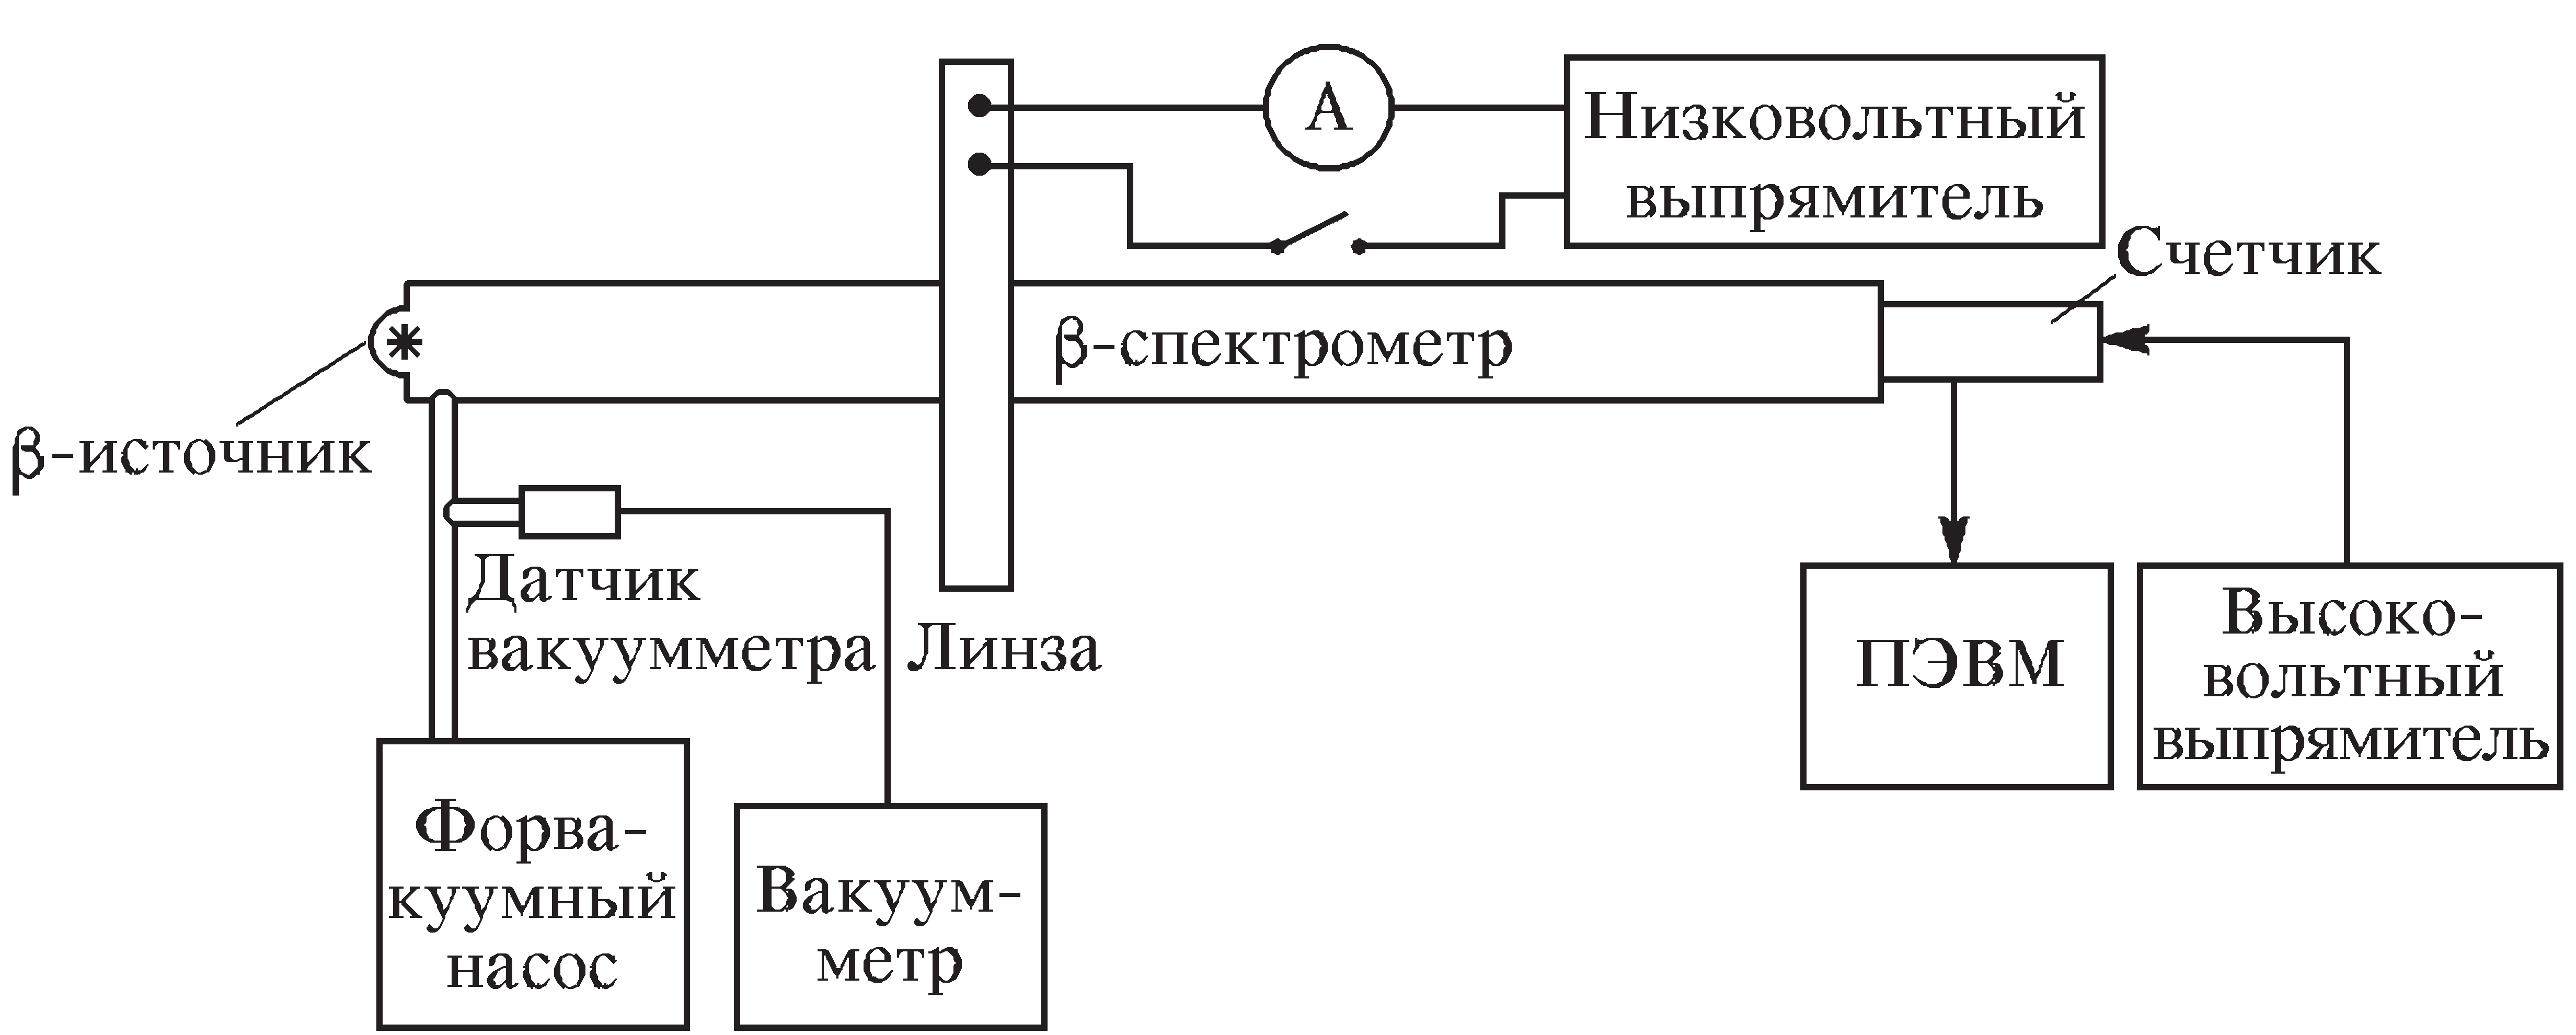
\includegraphics[width = 1\textwidth]{pics/ustan_2.png}
        \caption{Блок-схема установки для изучения $\beta$-спектра}
    \label{pic:ustan-2}
    \end{center}
\end{figure}
\FloatBarrier


Блок-схема установки для изучения $\beta$-спектров изображена на рис. \ref{pic:ustan-2}. Радиоактивный источник $\prescript{137}{}{\text{Cs}}$ помещен внутрь откачанной трубы. Электроны, сфокусированные магнитной линзой, попадают в счетчик. В газоразрядном счетчике они инициируют газовый разряд и тем самым приводят к появлению электрических импульсов на его электродах, которые затем регистрируются пересчетным прибором. В результате попадания электронов в сцинтиллятор на выходе фотоумножителя появляется электрические импульсы, которые заносятся в память персонального компьютера и выводятся на экран монитора. Давление в спектрометре поддерживается на уровне около 0,1 Тор и измеряется термопарным вакуумметром. Лучший вакуум в приборе не нужен, поскольку уже при этом давлении потери энергии электронов малы и их рассеяние незначительно. Откачка осуществляется форвакуумным насосом. Магнитная линза питается постоянным током от выпрямителя. Ток можно повышать до 6 А, он измеряется цифровым прибором. Высокое напряжение на ФЭУ или газоразрядный счетчик подается от стабилизированного выпрямителя.

\section{Результаты измерений и обработка данных}

\begin{enumerate}
    \item Откачаем воздух из спектрометра. Включим вакууметр и проверим его работу. Установим ток накала и включим режим измерения вакуума.
    \item Пока откачивается полость включим ПЭВМ и дождемся появления титульного листа программы.
    \item Включим формирователь импульсов, питание магнитной линзы и уменьшим ток до нуля.
    \item Проведем предварительное измерение спектра с шагом в 0.2 А до максимального тока в 4.4 А. Результаты измерения запишем в таблицу \ref{table:full_data}.
    \item Проведем подробное измерение конверсионного пика с шагом 0.05 А. Результаты измерения запишем в таблицу \ref{table:full_data}.
\end{enumerate}


\begin{table}[!ht]
    \centering
    \begin{tabular}{|l|r|r|cr|cr|cr|cr|}
        \hline
         & $I$, А & $N$, ч/с & $N'$ и $\sigma_{N'}$,  & ч/с & $p$ и $\sigma_p$,  & КэВ/с & $T$ и $\sigma_T$,  & КэВ&  $y_\text{ф}$ и $\sigma_\text{ф}$, &  $\text{КэВ}^{-3/2}$ \\ \hline
        0 & 0.20 & 1.4 & -0.6 & 0.2 & 62 & 2 & 3.8 & 0.2 & 0 & 0 \\
        1 & 0.40 & 1.2 & -0.8 & 0.2 & 125 & 2 & 15.0 & 0.4 & 0 & 0 \\
        2 & 0.60 & 1.2 & -0.8 & 0.2 & 187 & 2 & 33.2 & 0.5 & 0 & 0 \\
        3 & 0.80 & 2.6 & 0.6 & 0.2 & 250 & 2 & 57.7 & 0.7 & 200 & 38 \\
        4 & 1.00 & 4.9 & 2.9 & 0.3 & 312 & 2 & 87.7 & 0.8 & 312 & 15 \\
        5 & 1.20 & 8.8 & 6.8 & 0.3 & 374 & 2 & 122.4 & 0.9 & 360 & 9 \\
        6 & 1.40 & 12.5 & 10.5 & 0.4 & 437 & 2 & 161.1 & 1.0 & 355 & 7 \\
        7 & 1.60 & 13.8 & 11.8 & 0.4 & 499 & 2 & 203.2 & 1.1 & 308 & 6 \\
        8 & 1.80 & 14.5 & 12.5 & 0.4 & 561 & 2 & 248.1 & 1.2 & 267 & 5 \\
        9 & 2.00 & 15.6 & 13.6 & 0.4 & 624 & 2 & 295.4 & 1.2 & 237 & 4 \\
        10 & 2.20 & 13.7 & 11.7 & 0.4 & 686 & 2 & 344.5 & 1.3 & 190 & 3 \\
        11 & 2.40 & 12.5 & 10.5 & 0.4 & 749 & 2 & 395.3 & 1.3 & 158 & 3 \\
        12 & 2.60 & 7.4 & 5.4 & 0.3 & 811 & 2 & 447.5 & 1.3 & 101 & 3 \\
        13 & 2.80 & 4.5 & 2.5 & 0.3 & 873 & 2 & 500.8 & 1.3 & 62 & 3 \\
        14 & 3.00 & 3.8 & 1.8 & 0.3 & 936 & 2 & 555.1 & 1.4 & 46 & 3 \\
        15 & 3.05 & 8.0 & 6.0 & 0.3 & 951 & 2 & 568.8 & 1.4 & 83 & 2 \\
        16 & 3.10 & 13.0 & 11.0 & 0.4 & 967 & 2 & 582.6 & 1.4 & 110 & 2 \\
        17 & 3.15 & 19.6 & 17.6 & 0.5 & 982 & 2 & 596.4 & 1.4 & 136 & 2 \\
        18 & 3.20 & 22.8 & 20.8 & 0.5 & 998 & 2 & 610.3 & 1.4 & 145 & 2 \\
        19 & 3.25 & 26.2 & 24.2 & 0.5 & 1014 & 2 & 624.2 & 1.4 & 152 & 2 \\
        20 & 3.30 & 23.9 & 21.9 & 0.5 & 1029 & 2 & 638.1 & 1.4 & 142 & 2 \\
        21 & 3.35 & 18.4 & 16.4 & 0.5 & 1045 & 2 & 652.1 & 1.4 & 120 & 2 \\
        22 & 3.40 & 14.5 & 12.5 & 0.4 & 1060 & 2 & 666.1 & 1.4 & 102 & 2 \\
        23 & 3.45 & 10.3 & 8.3 & 0.4 & 1076 & 2 & 680.2 & 1.4 & 82 & 2 \\
        24 & 3.50 & 6.2 & 4.2 & 0.3 & 1092 & 2 & 694.3 & 1.4 & 57 & 2 \\
        25 & 3.60 & 2.0 & 0.0 & 0.2 & 1123 & 2 & 722.6 & 1.4 & 4 & 22 \\
        26 & 3.80 & 0.8 & -1.2 & 0.2 & 1185 & 2 & 779.7 & 1.4 & 0 & 0 \\
        27 & 4.00 & 0.7 & -1.3 & 0.2 & 1248 & 2 & 837.2 & 1.4 & 0 & 0 \\
        28 & 4.20 & 0.6 & -1.4 & 0.2 & 1310 & 2 & 895.1 & 1.5 & 0 & 0 \\
        29 & 4.40 & 0.5 & -1.5 & 0.2 & 1372 & 2 & 953.4 & 1.5 & 0 & 0 \\ \hline
        \end{tabular}
    \caption{Измерения спектра и пересчет промежуточных значений}
    \label{table:full_data}
\end{table}



\begin{enumerate}[resume]
    \item Измерим фон и запишем в таблицу \ref{table:background}. Измерения произведем при минимальном и максимальном значении тока.
\end{enumerate}

\begin{table}[!ht]
    \centering
    \begin{tabular}{|l|c|c|c|}
         \hline
         $t$, с & $I$, А & $N_f$, ч/с & $\sigma_{N_f}$, ч/с \\ \hline
         100    & 0.00   & 1.3        & 0.1                 \\ \hline
         100    & 3.25   & 0.8        & 0.1                 \\ \hline
    \end{tabular}
    \caption{Измерение фонового $\beta$-излучения}
    \label{table:background}
\end{table}



\begin{enumerate}[resume]
    \item Обработка результатов.
\end{enumerate}

Учтем фон при измерениях. Возьмем значение фона при $I = 0.00$ А. Новое значение числа частиц $N' = N - N_F$. Заметим, что часть значений стала отрицательной. Будем считать, что они вызваны исключительно фоновым излучением и не учитывать их при финальных вычислениях. Все промежуточные вычисления записываем в таблицу \ref{table:full_data}.

Прокалибруем спектрометр с учетом того, что величина $p_e c = 1013.5$ КэВ для конверсионного электрона:

\begin{equation*}
    p_e = k I, p_e c = E_{cal} = 1013.5 \ \text{КэВ} \implies k = \cfrac{p_e}{I} = \cfrac{E_{cal}}{c I}
\end{equation*}

\newpage

Погрешность вычисления $k$:

\begin{multline*}
    \sigma_k = \sqrt{ \left( \cfrac{\partial k}{\partial c} \right)^2 \sigma_c^2 + \left( \cfrac{\partial k}{\partial E_{cal}} \right)^2 \sigma_{E_{cal}}^2 + \left( \cfrac{\partial k}{\partial I} \right)^2 \sigma_I^2 } = \\ = \sqrt{ \left( - \cfrac{k}{c} \right)^2 \sigma_c^2 + \left( - \cfrac{k}{E_{cal}} \right)^2 \sigma_{E_{cal}}^2 + \left( - \cfrac{k}{I} \right)^2 \sigma_I^2 } = \\ = k \sqrt{ \left( \cfrac{\sigma_c}{c} \right)^2 + \left( \cfrac{\sigma_{E_{cal}}}{E_{cal}} \right)^2 + \left( \cfrac{\sigma_I}{I} \right)^2 }
\end{multline*}

Тогда $k = (311.85 \pm 0.02) \ \text{КэВ}\cdot \text{с}^{-1} / \text{А}$ 


Погрешность пересчета $p = kI$ вычисляется по формуле: $\sigma_p = p \sqrt{(\sigma_I / I)^2 + (\sigma_k / k)^2}$. Посчитаем все $p$ и их погрешности и запишем в таблицу \ref{table:full_data}.


Для построения графика Ферми-Кюри нужно вычислить кинетическую энергию электронов ($p$ в КэВ/с):

\begin{equation*}
    T = c\sqrt{(p/c)^2 + m_e^2 c^2} - m_e c^2 = \sqrt{ \left(p\right)^2 + \left(m_e c^2\right)^2} - m_e c^2
\end{equation*}

И погрешность:

\begin{equation*}
    \sigma_T = \left| \frac{\partial T}{\partial p} \right| \sigma_p = \frac{ p\sigma_p}{\sqrt{\left(p\right)^2 + \left(m_e c^2\right)^2}}
\end{equation*}

где $c = 299792458$ м/с, $m_e c^2 = 511.2$ КэВ.

Посчитаем энергии и погрешности и запишем в таблицу \ref{table:full_data}.


Далее вычислим координаты Ферми:

\begin{equation*}
    x_\text{ф} = T, \ \ \ y_\text{ф} = \cfrac{\sqrt{N'(p)}}{p^{3/2}} \cdot 10^6
\end{equation*}

Погрешность $\sigma_{x_\text{ф}} = \sigma_T$, а погрешность $\sigma_{y_\text{ф}}$ вычислим через частные производные:

\begin{equation*}
    \sigma_{y_\text{ф}} = \sqrt{ \left( \cfrac{\partial y_\text{ф}}{\partial N} \right)^2 \sigma_N^2 + \left( \cfrac{\partial y_\text{ф}}{\partial p_e} \right)^2 \sigma_{p_e}^2 }  = \sqrt{ \left( \cfrac{y_\text{ф}}{2N}   \right)^2 \sigma_N^2 + \left( -\cfrac{3}{2} \cfrac{y_\text{ф}}{p_e}  \right)^2 \sigma_{p_e}^2 } = \frac{1}{2} y_\text{ф} \sqrt{\left(\cfrac{\sigma_N}{N}\right)^2 + \left(\cfrac{3\sigma_{p_e}}{p_E}\right)^2}
\end{equation*}

Посчитаем их и запишем в таблицу \ref{table:full_data}.

\begin{enumerate}[resume]
    \item Построим график Ферми-Кюри на рис. \ref{plot:fermi}
\end{enumerate}

Аппроксимируем прямую линию \[ \frac{\sqrt{N'(p)}}{p} \approx T - E_e \implies \frac{\sqrt{N'(p)}}{p} = a\cdot T + b \]

Коэффициенты прямой:

\begin{equation*}
    a = -(0.79 \pm 0.03) \ \  \text{КэВ}^{-1} \cdot \text{эВ}^{-1}, \ \ \ b = (466 \pm 9) \ \ \text{эВ}^{-1}
\end{equation*}

Энергию $E_e$ тогда можно вычислить по формуле: $E_e = - b / a$, с погрешностью 
\[\sigma_{E_e} = E_e \sqrt{(\sigma_a / a)^2 + (\sigma_b / b)^2}\].

\[E_e = (592 \pm 22) \ \text{КэВ}\]

\FloatBarrier
\begin{figure}[!ht]
	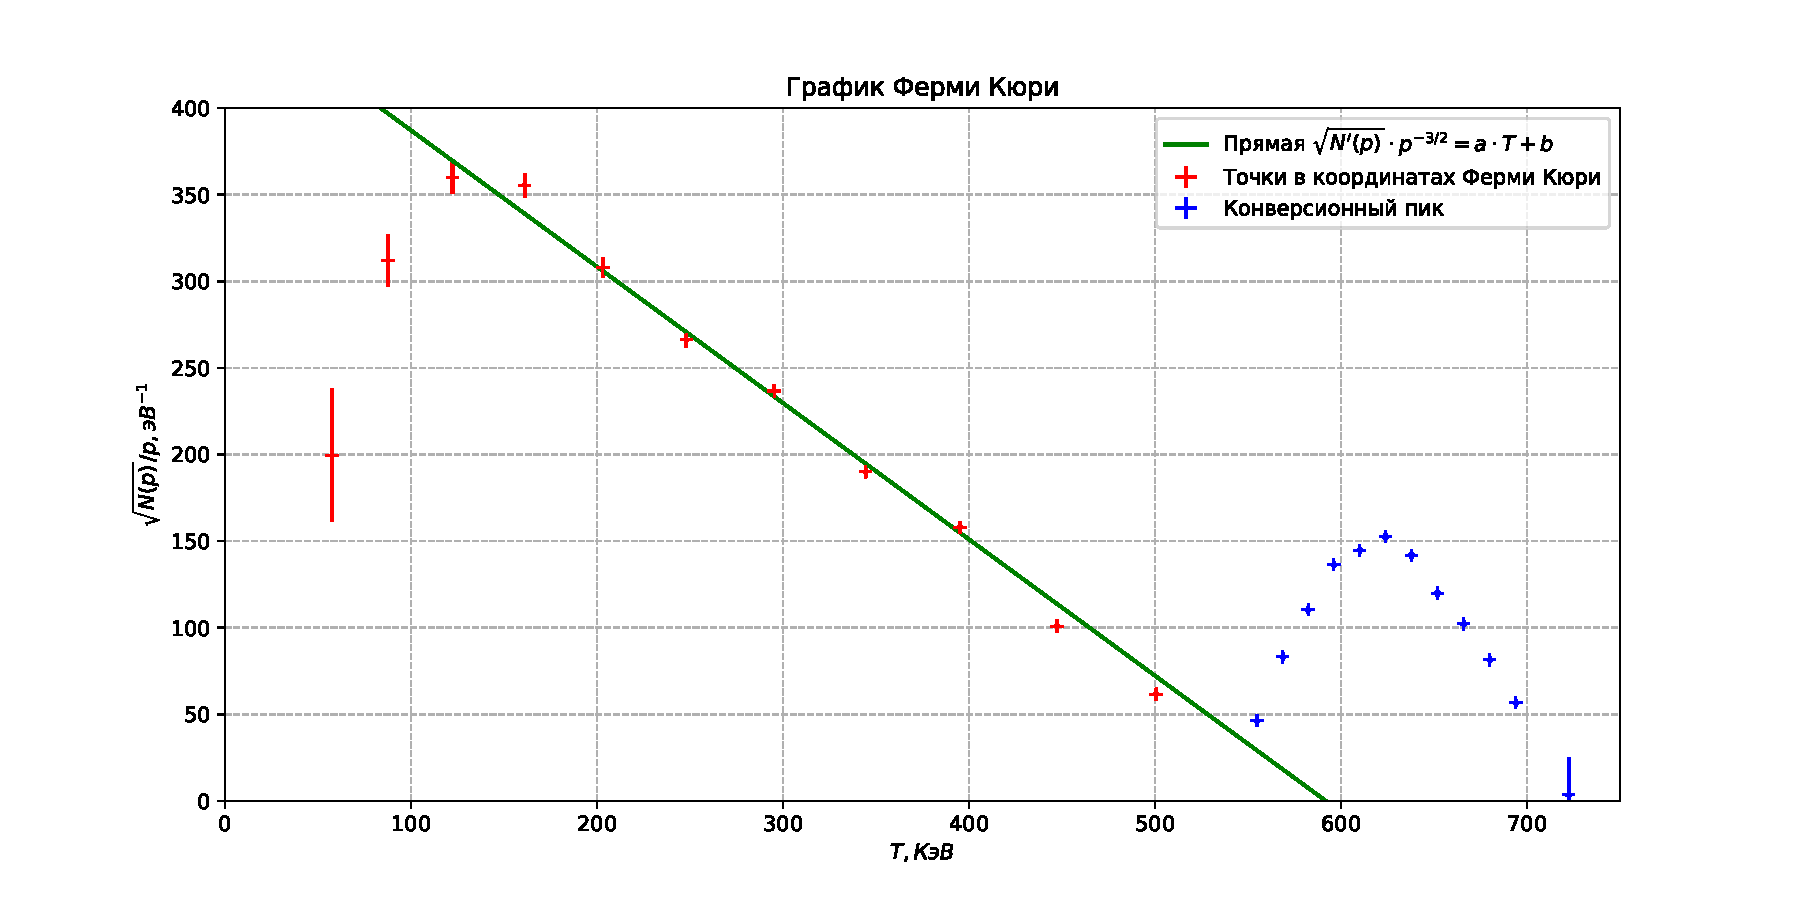
\includegraphics[width=1.1\textwidth]{plots/plot_fermi.pdf}
	\caption{\textit{График Ферми-Кюри}}
	\label{plot:fermi}
\end{figure}
\FloatBarrier

\begin{enumerate}[resume]
    \item Построим график спектра по энергиям (рис. \ref{plot:T_N}) и попробуем аппроксимировать его.
\end{enumerate}

\FloatBarrier
\begin{figure}[!ht]
	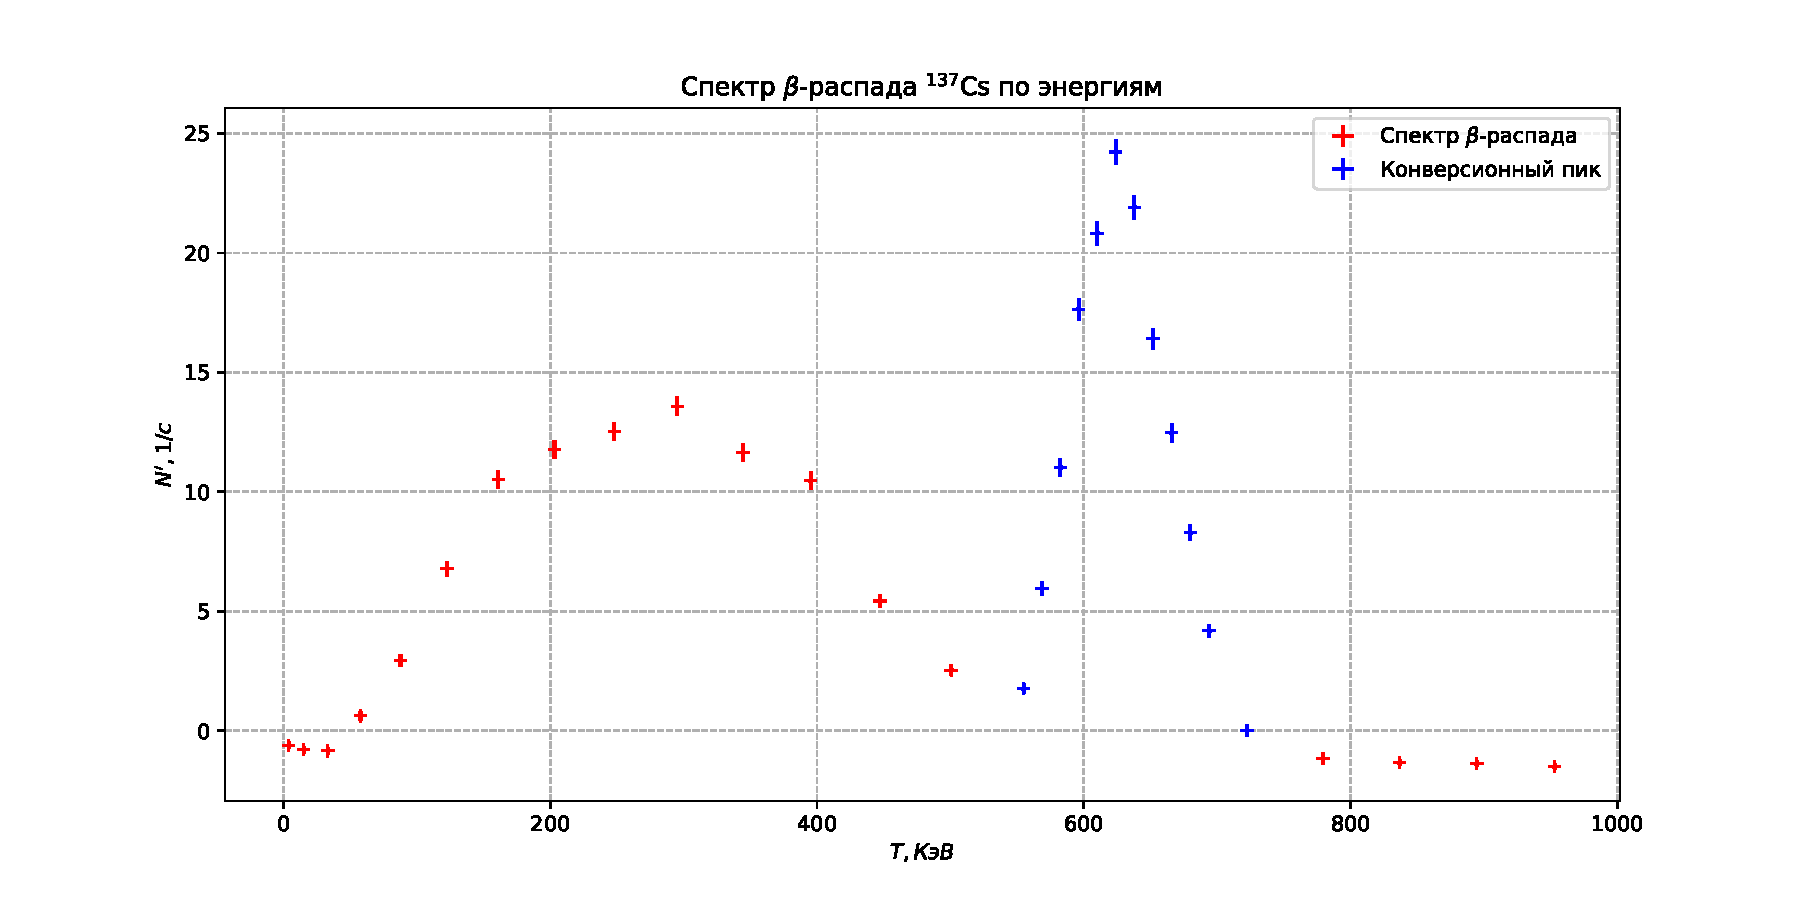
\includegraphics[width=1.1\textwidth]{plots/T_N.pdf}
	\caption{\textit{Энергетический спектр $\beta$-распада $\prescript{137}{}{\text{Cs}}$}}
	\label{plot:T_N}
\end{figure}
\FloatBarrier

\newpage

Попробуем отделить два пика и аппроксимировать каждый функцией гаусса.

Для основного спектра $N_1(T)$, а для конверсионного пика $N_2(T)$:

\begin{equation*}
    N_i(T) = a_i \cdot \exp{\left( - \frac{(T - \mu_i)^2}{2 \sigma_i^2} \right)} + b_i
\end{equation*}

\begin{table}[!ht]
    \centering
    \begin{tabular}{|l|l|l|l|l|l|l|l|l|}
    \hline
      & $a_i$  & $\sigma_{a_i}$ & $\mu_i$  & $\sigma_{\mu_i}$ & $\sigma_i$ & $\sigma_{\sigma_i}$ & $b_i$    & $\sigma_{b_i}$ \\ \hline
    1 & 16 & 1        & 284 & 5         & 131   & 7            & -1.8 & 0.5      \\ \hline
    2 & 24 & 1        & 626 & 1         & -37   & 2            & -1   & 1        \\ \hline
    \end{tabular}
    \caption{Коэффициенты для аппроксимаций спектра функциями Гаусса}
    \label{table:gauss_coefs}
\end{table}

аппроксимируем по правилу: \[ 
N(T) =
\begin{cases}
N_1(T), \ T \leq 500 \ \text{КэВ}  \\
\left(2.5 \cdot N_1(T) + N_2(T)\right) / 2, \ T \leq 550 \ \text{КэВ}  \\
N_2(T), \ \ \text{при всех остальных} \ T 
\end{cases}
\]

И изобразим на рис. \ref{plot:T_N_gauss}.

\FloatBarrier
\begin{figure}[!ht]
	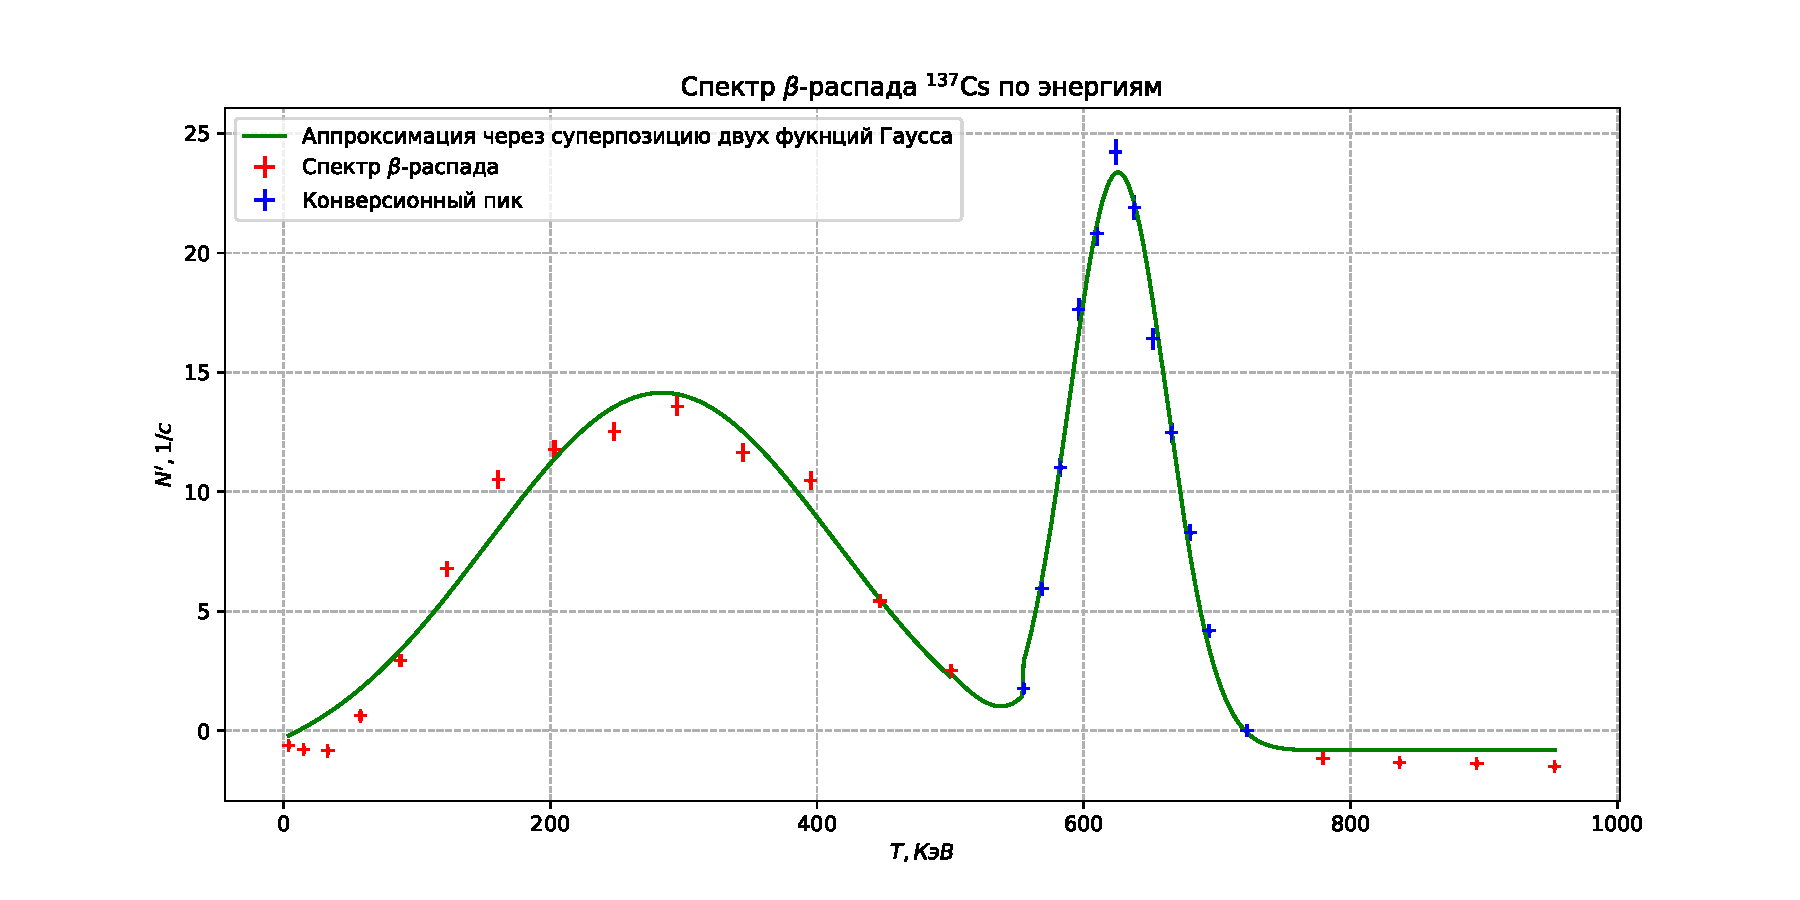
\includegraphics[width=1.1\textwidth]{plots/T_N_gaus_model.pdf}
	\caption{\textit{Энергетический спектр $\beta$-распада $\prescript{137}{}{\text{Cs}}$ с аппроксимацией по Гауссу}}
	\label{plot:T_N_gauss}
\end{figure}
\FloatBarrier

\begin{enumerate}[resume]
    \item Аппроксимируем спектр с помощью нейронной сети.
\end{enumerate}

Сначала подготовим данные для обучения. Сначала проведем интерполяцию данных энергии и числа частиц, где между каждыми двумя точками добавим еще 3 точки. Далее сделаем столбец, где 0, если точка не принадлежит конверсионному пику, а 1 - если принадлежит. Сделаем два столбца с расстоянием до центра спектра и до центра конверсионного пика. И два столбца со 2, 3 и 4 степенью энергии. Так же два столбца со значениями $N_1(T)$ и $N_2(T)$.

\newpage

С помощью StandardScaler нормируем данные. Итого получаем 9 признаков и в качестве target $N'$.


Нейронная сеть имеет в первом слое 128 нейронов, 128 во втором, 64 в третьем и и 32 в последнем. В качестве функции активации используем сигмоиду. Функция оптимизатор - МНК. Обучим нейросеть до значения МНК < 0.5. Изобразим график предсказания на рис. \ref{plot:T_N_nn}.

\FloatBarrier
\begin{figure}[!ht]
	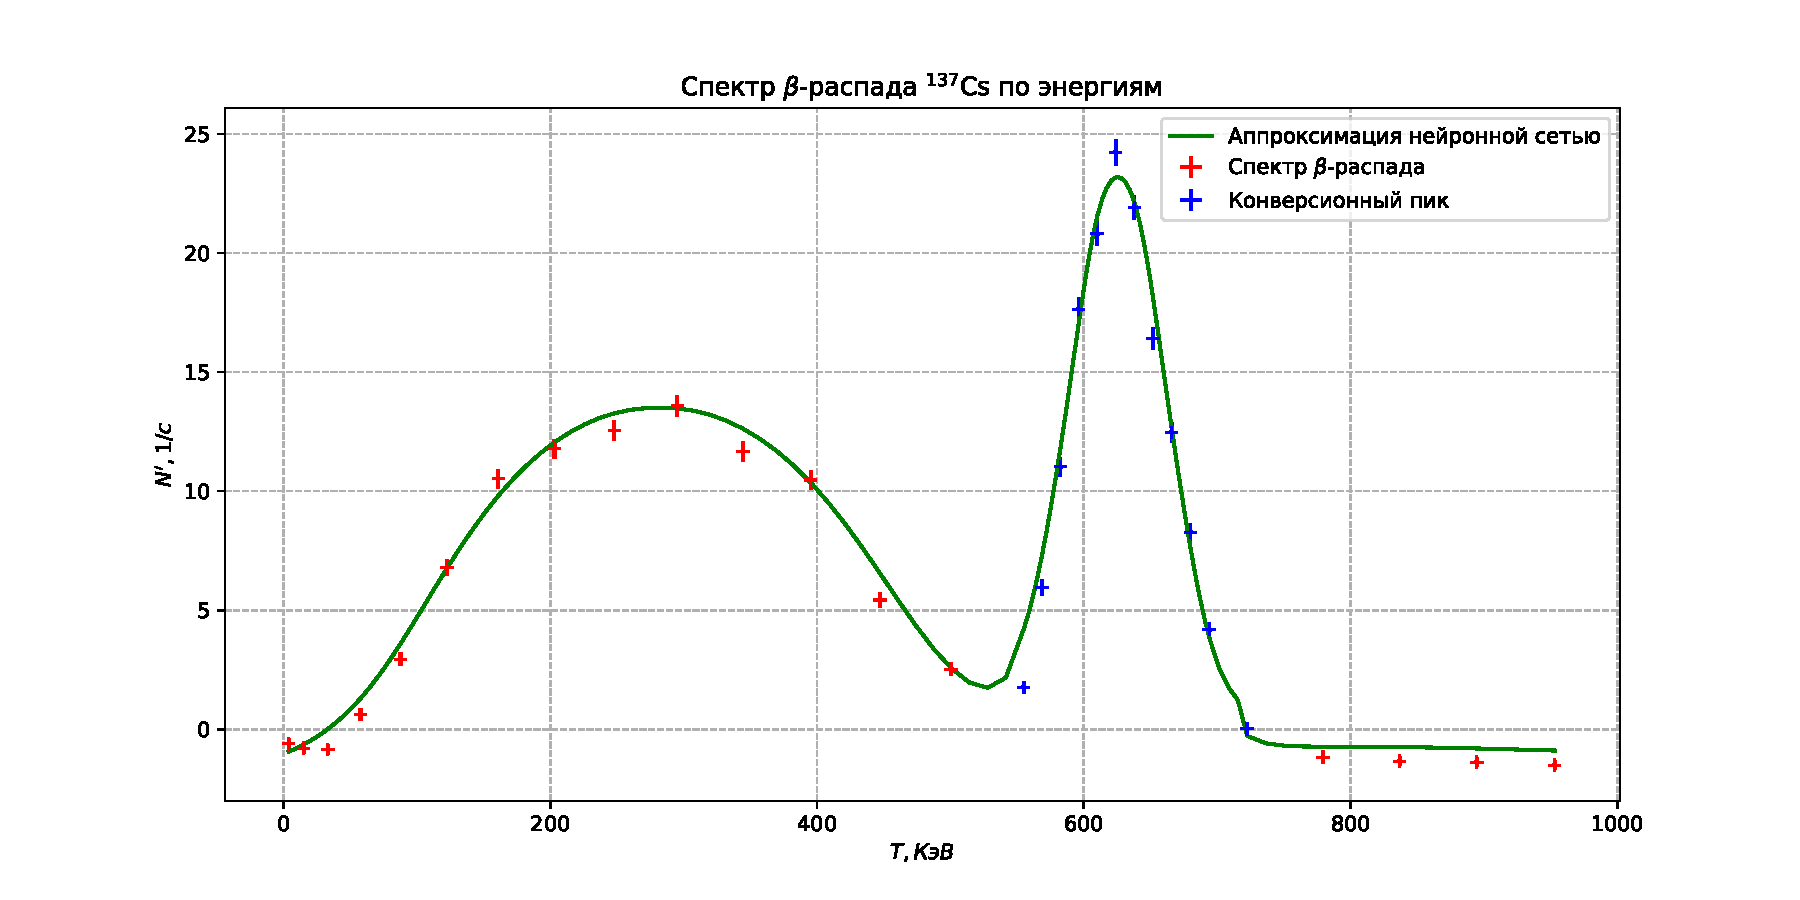
\includegraphics[width=1.1\textwidth]{plots/T_N_nn.pdf}
	\caption{\textit{Энергетический спектр $\beta$-распада $\prescript{137}{}{\text{Cs}}$ с аппроксимацией нейронноя сетью}}
	\label{plot:T_N_nn}
\end{figure}
\FloatBarrier


\section{Выводы}

\begin{enumerate}
    \item Был исследован спектр $\beta$-частиц при распаде ядер $\prescript{127}{}{\text{Cs}}$.
    \item Была определена энергия $E_e$.
\end{enumerate}



\end{document}
